% Teilaufgabe 1

\section{Normale und anormale Dispersion}
\label{sec:dispersion}

\paragraph*{Normale Dispersion: }
Mit zunehmender Wellenlänge sinkt der Brechungsindex. (Reeller Anteil)

\paragraph*{Annormale Dispersion: }
Mit zuhnemender Wellenlänge steiget der Brechungsindex. (Imaginärer Anteil)

\begin{figure}[h]
    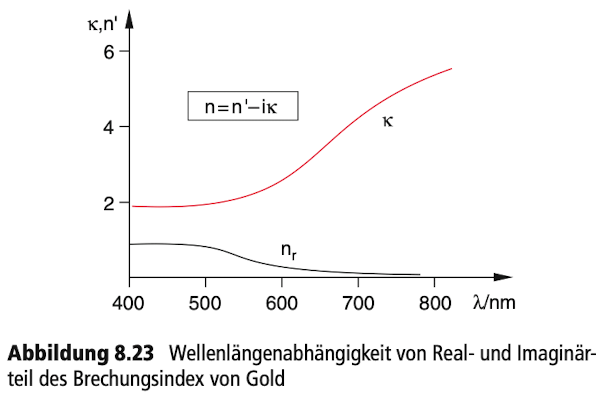
\includegraphics[width=0.95\textwidth]{Bilder/Dispersion.png}
    \caption{Dispersionrelation, entnommen aus Demtröder, Elektrizität und Optik, Auflage 6 (2013).}
\end{figure}